\section{Force calculation}

\begin{frame}
    \frametitle{$F_{ij} = -F_{ji}$}
        \textbf{Task:} Implement Force calculation with the pairwise iterator

        \textbf{Solution:} Skip calculations due to $F_{ij} = -F_{ji}$
        \vspace{-15pt}
        \begin{equation}
            F_i = \sum_{j=1, j \neq i}^{\#particles} F_{i,j}
        \end{equation}
        \vspace{-15pt}
        \begin{align}
            F_{i,j} &= \frac{m_im_j}{(||x_i-x_j||_2)^3} (x_j - x_i) \\
                    &= \frac{m_jm_i}{(||x_j-x_i||_2)^3} \left(-1 \cdot \left(x_i - x_j\right)\right) = - F_{j,i}
        \end{align}
\end{frame}

\begin{frame}
    \frametitle{Force calculation}
    \begin{columns}
        \begin{column}{0.5\textwidth}
            \begin{table}[H]
                \begin{tabular}{|l|l|l|l|l|}
                \hline
                    & Time for $10^6$ iterations \\ \hline
                Naive & 31109ms                  \\ \hline
                V2    & 24881ms                  \\ \hline
                \end{tabular}
                \caption{Values measured for the two different force calculation strategies. Approx speedup of 1.25.}
                \label{tab:speedup}
            \end{table}
        \end{column}
        \begin{column}{0.5\textwidth}
            \begin{figure}[]
                \centering
                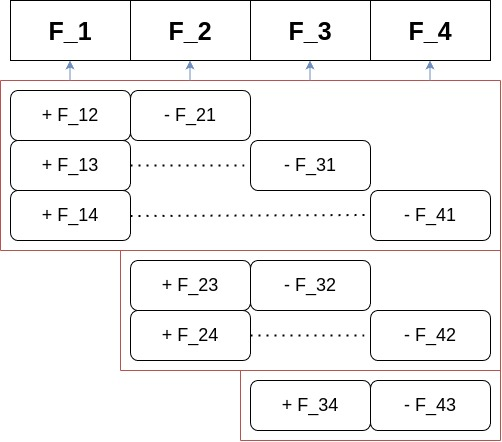
\includegraphics[width=\columnwidth]{ForceCalcFig.jpg}
                \caption{Pairwise Addition of Forces}
            \end{figure}
        \end{column}
    \end{columns}
\end{frame}